\documentclass{article}
\usepackage{amsmath, amsthm, amssymb}
\usepackage{listings, xcolor}
\usepackage{graphicx}
\usepackage[pdfborder=000]{hyperref}
\usepackage{subfig}

\title{Report to Project-4}
\author{Yuanbo Han\quad15300180032}
\date{December 30, 2017}

\graphicspath{{figures/}}

\lstset{
	columns=fixed,
	numbers=left,
	frame=none,
	keywordstyle=\color[RGB]{40,40,255},
	numberstyle=\footnotesize\color{darkgray},
	commentstyle=\it\color[RGB]{0,96,96},
	stringstyle=\rmfamily\slshape\color[RGB]{128,0,0},
	showstringspaces=false,
	language=Matlab,
}

\begin{document}
\maketitle
\tableofcontents

\section{Dimensionality Reduction}
\subsection{PCA}
\subsubsection{Choice for $k$}
\label{sec-1.1.1}
I write the script $select\_k.m$ to read data, convert to double, plot the eigen spectra, and select $k$. \hyperref[fig-1]{Figure~1} shows the eigen spectra of $XX^T/N$ with first removing the mean.

\begin{figure}
	\centering
	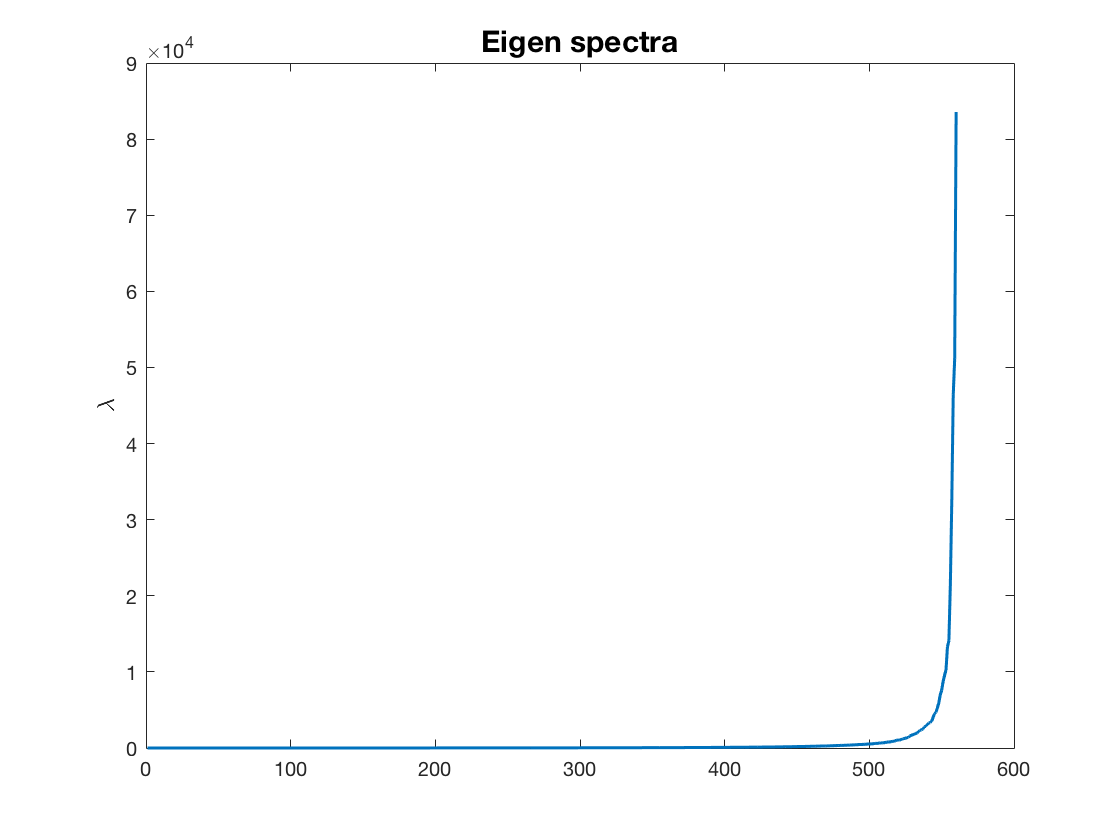
\includegraphics[scale=0.3]{eigenspectra.png}
	\caption{Eigen Spectra}
	\label{fig-1}
\end{figure}

We can observe that only a few eigen values are big, whereas the vast majority are small enough to be omitted. Such being the case, we conclude the main information of pictures are stored in those big eigen values. And therefore, discarding the small ones not only reduces the storage required for saving pictures, but also does good to denoising.

The retention rate of PCA can be defined as
\[
rate = \frac{\sum_{i=560-k+1}^{560} \lambda_i}{\sum_{j=1}^{560} \lambda_j}
\]
Thus we select $k$ based on our expected retention rate. For example, $k=80$ at the retention rate of $95\%$, and $k=20$ at $80\%$. As my own preference, $k=80$ is a reasonable choice.

\subsubsection{Visualize Eigenvectors}
\hyperref[fig-2]{Figure~2}, plotted by the script $showEigenvectors.m$, shows the top 16 eigenvectors with and without first removing the mean. As we can see, each picture characterizes certain features of the original photo, such as the eyes, brow, nose, mouth, moustache and so on. The features showed in each of group are in general corresponding to one of the other group. But the difference is, pictures in \hyperref[subfig-2(b)]{Figure~2(b)} (with first removing the mean) specifies the details more distinctly than those in \hyperref[subfig-2(a)]{Figure~2(a)}. In conclusion, it is effective and efficient to first remove the mean.

\begin{figure}
	\centering
	\subfloat[Mean Not Removed]{\label{subfig-2(a)}
		\centering
		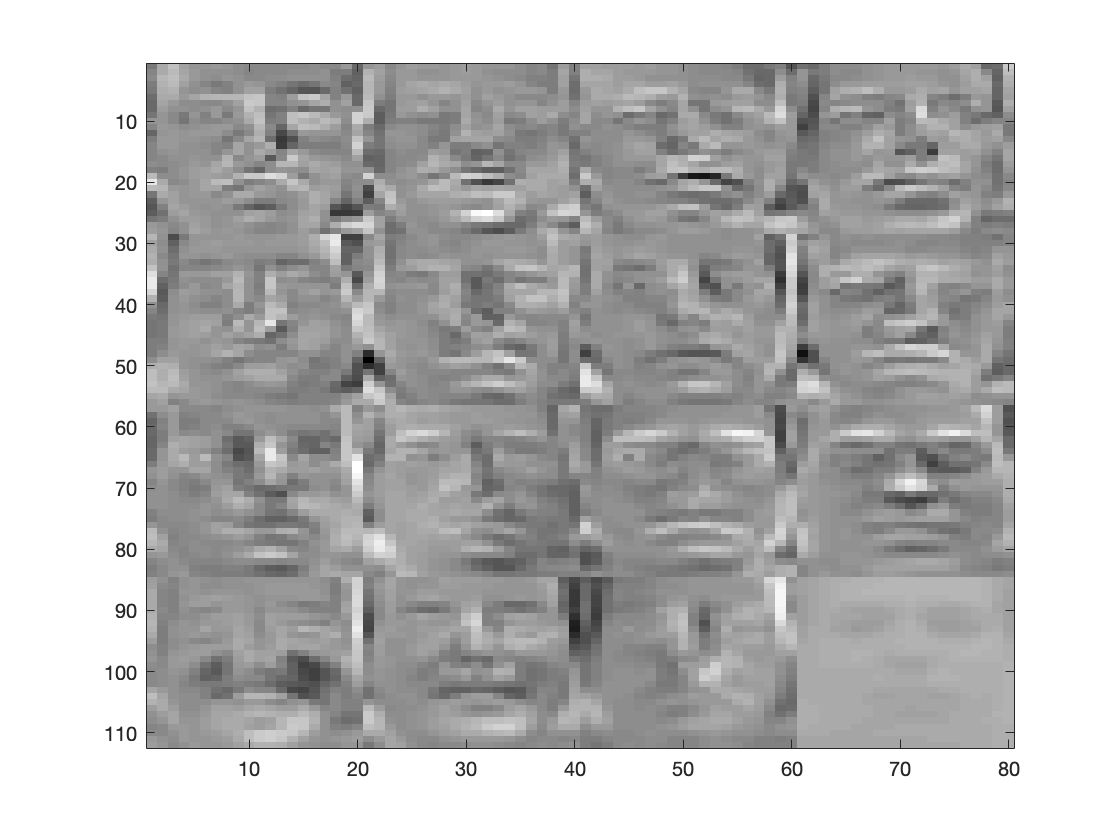
\includegraphics[scale=0.14]{2un.png}
	}
	\quad
	\subfloat[Mean Removed]{\label{subfig-2(b)}
		\centering
		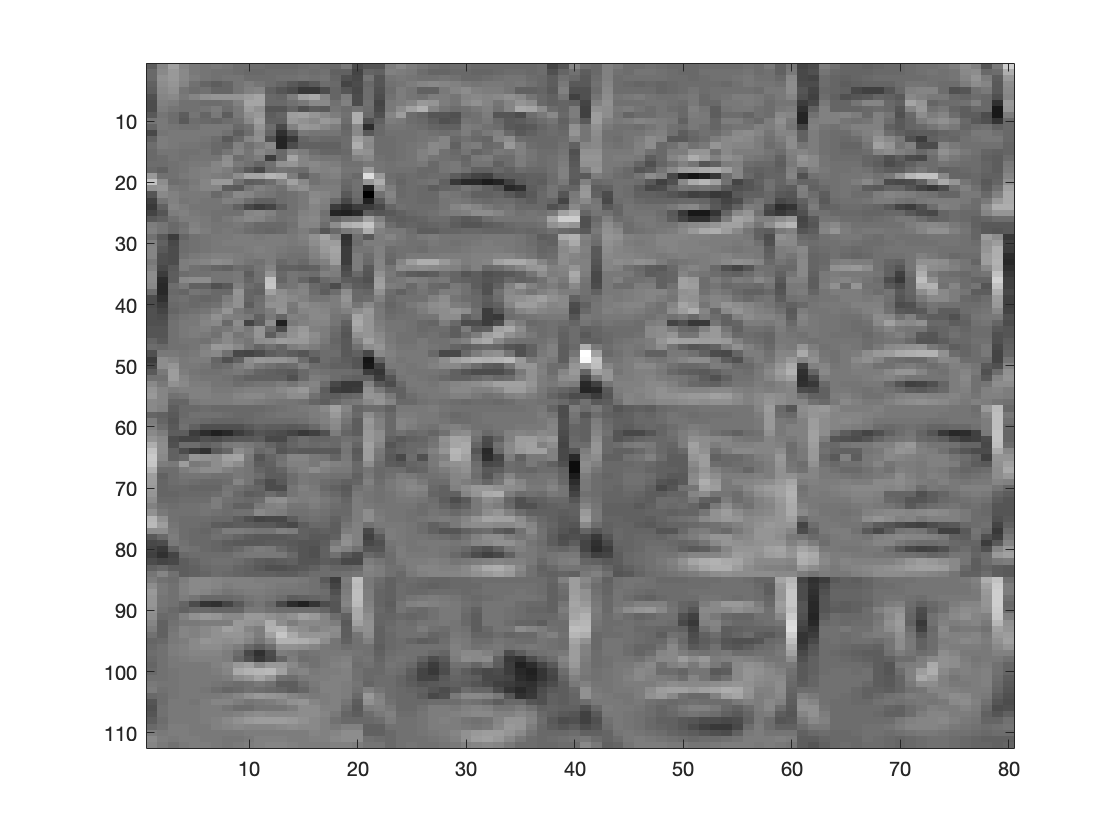
\includegraphics[scale=0.14]{2ctr.png}
	}
	\caption{The Top 16 Eigenvectors}
	\label{fig-2}
\end{figure}

\subsubsection{Project onto 2D}
The script $projectOnto2D.m$ projects data onto the top two eigenvectors, and plots the resulting 2D points (\hyperref[fig-3]{Figure~3}). As a consequence, the projection makes little sense since the outcome points comes too close to each other. The reason is evident---setting $k=2$ loses too much information of the original pictures. Recall that in \hyperref[sec-1.1.1]{Section~1.1.1}, we have discussed how to select $k$.
\begin{figure}
	\centering
	\subfloat[Mean Not Removed]{\label{subfig-3(a)}
		\centering
		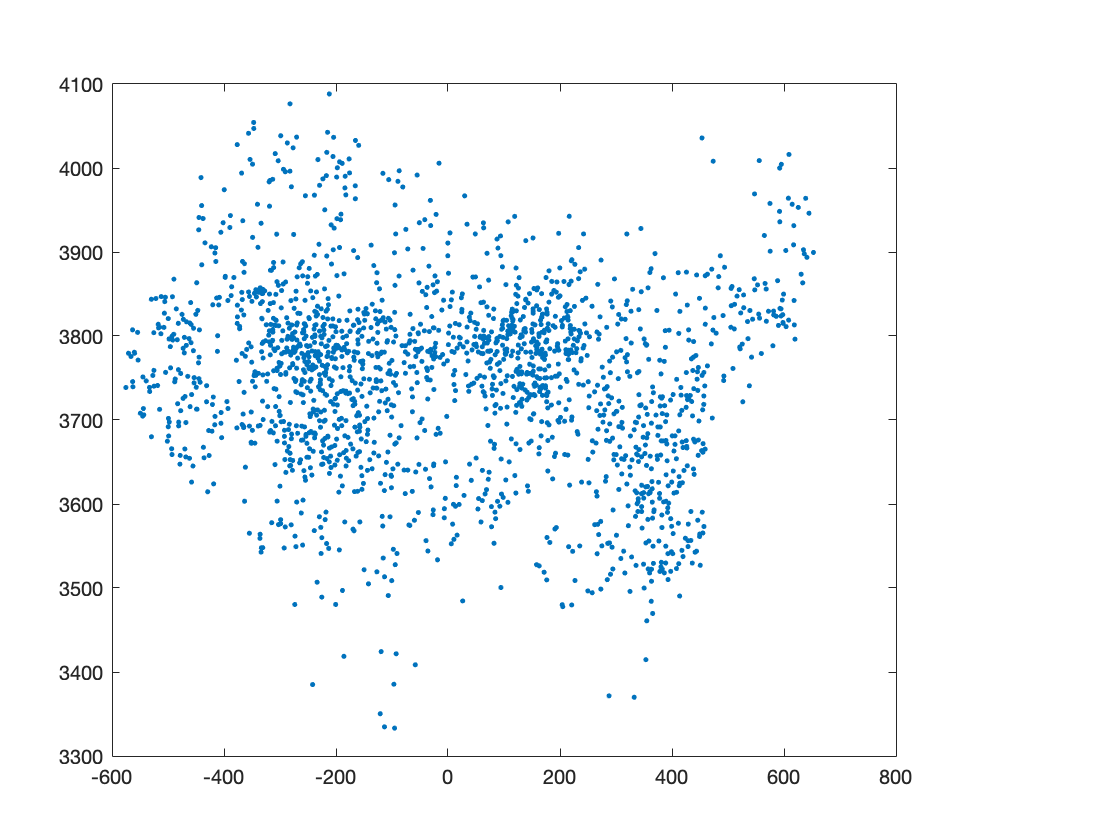
\includegraphics[scale=0.14]{3un.png}
	}
	\quad
	\subfloat[Mean Removed]{\label{subfig-3(b)}
		\centering
		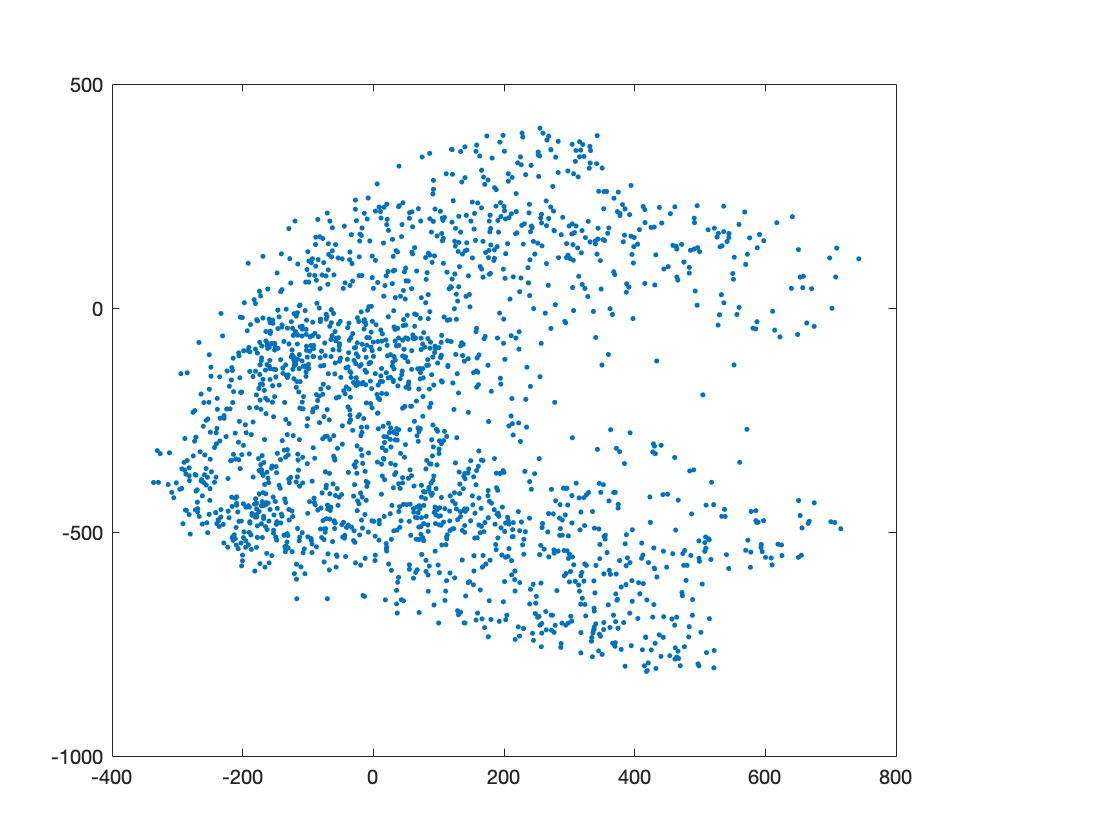
\includegraphics[scale=0.14]{3ctr.png}
	}
	\caption{Project onto 2D}
	\label{fig-3}
\end{figure}

\subsubsection{Reconstruction}
\label{sec-1.1.4}
My function $PCAreconstruct$ compose the corresponding projected vector of Y, where V is the eigenvectors used in PCA.

As discussed before, we select $k=80$ at the retention rate of $95\%$, and use first remove the mean. For the sake of comparison, my script $showReconstruct.m$ plots both the original picture to be processed, and the reconstructed one. Take an informative picture from the data and a randomly generated data as examples, the results are in \hyperref[fig-4]{Figure~4} and \hyperref[fig-5]{Figure~5}.

\begin{figure}
	\centering
	\subfloat[Original]{
		\centering
		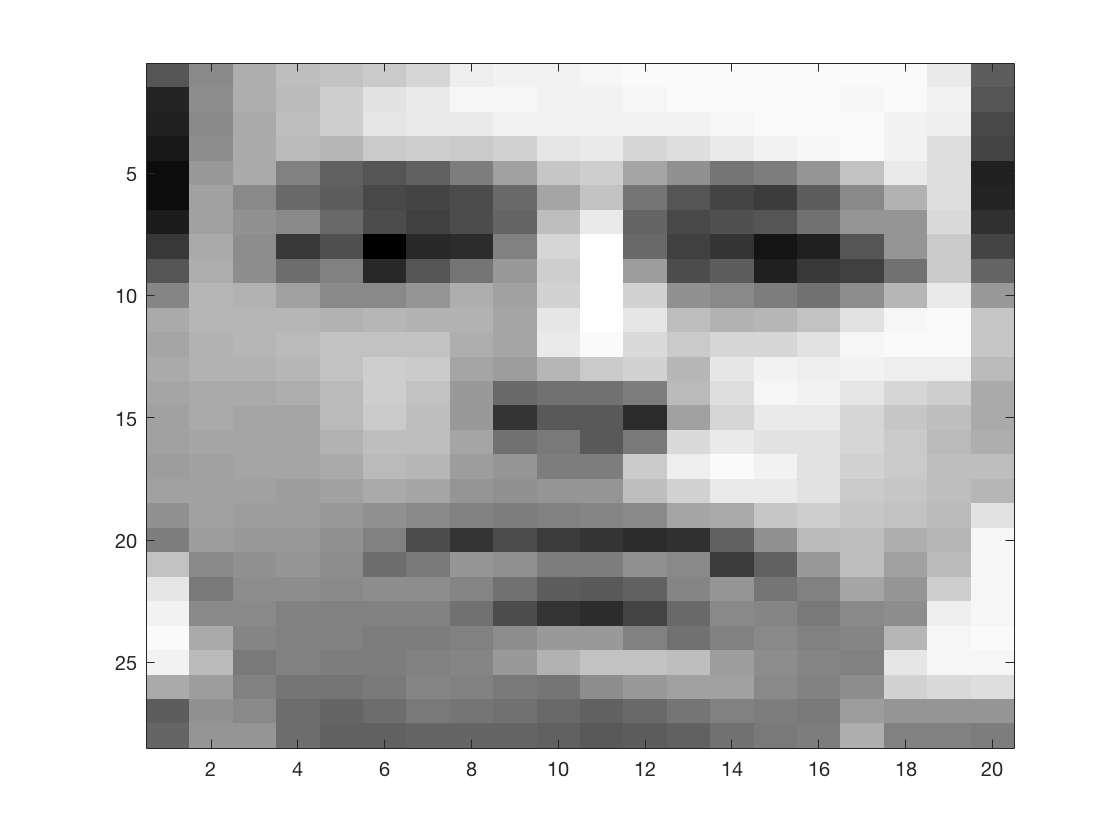
\includegraphics[scale=0.14]{4orig.png}
	}
	\quad
	\subfloat[Reconstructed]{
		\centering
		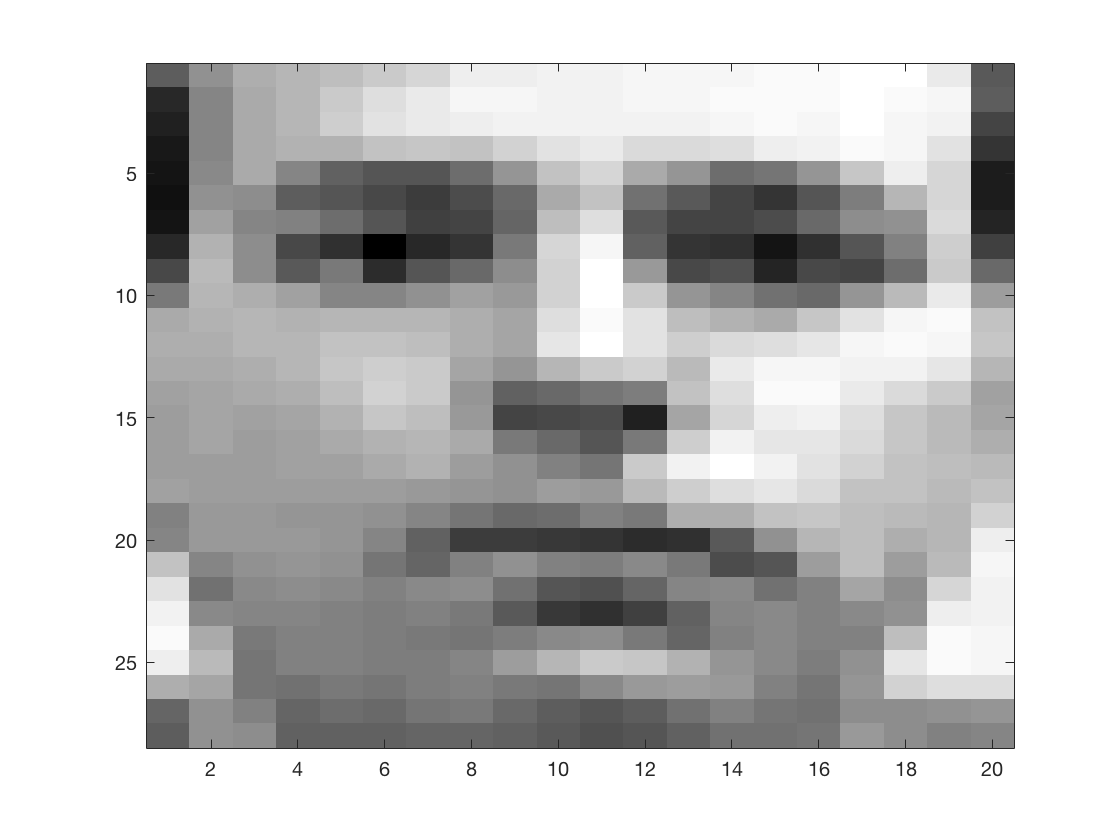
\includegraphics[scale=0.14]{4orig_re.png}
	}
	\caption{An Informative Example}
	\label{fig-4}
\end{figure}

\begin{figure}
	\centering
	\subfloat[Original]{
		\centering
		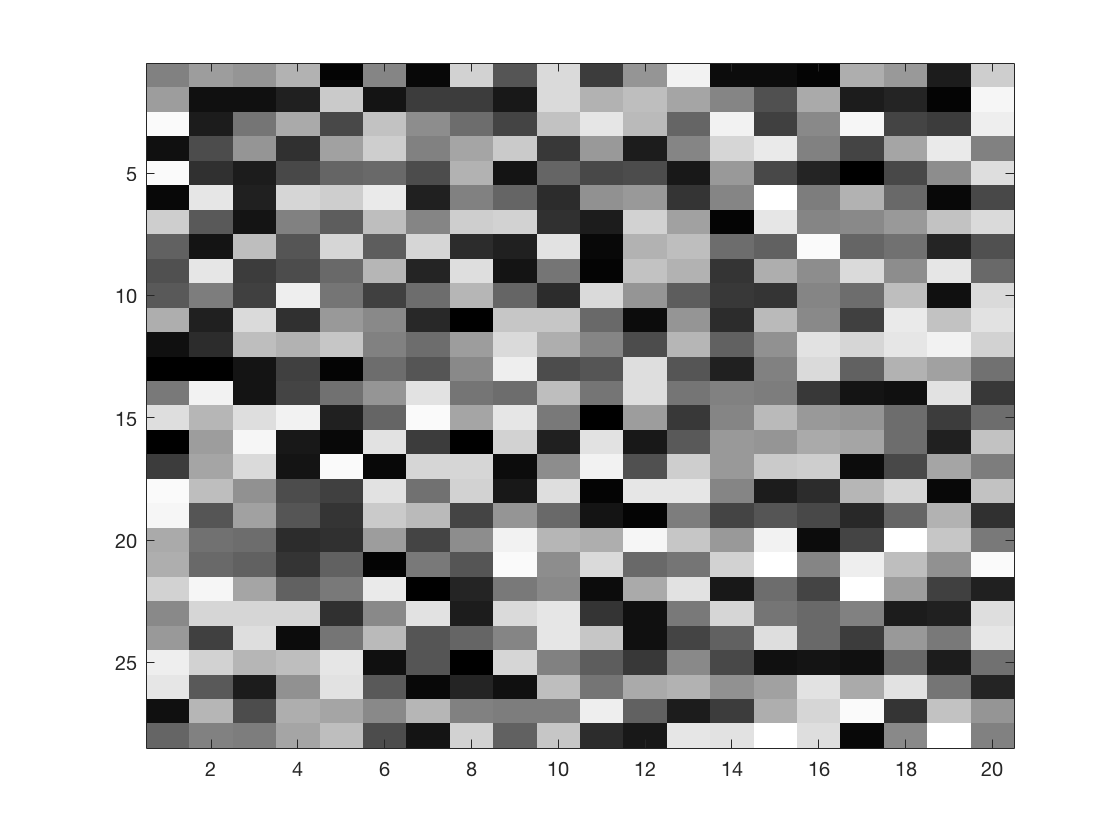
\includegraphics[scale=0.14]{4rand.png}
	}
	\quad
	\subfloat[Reconstructed]{
		\centering
		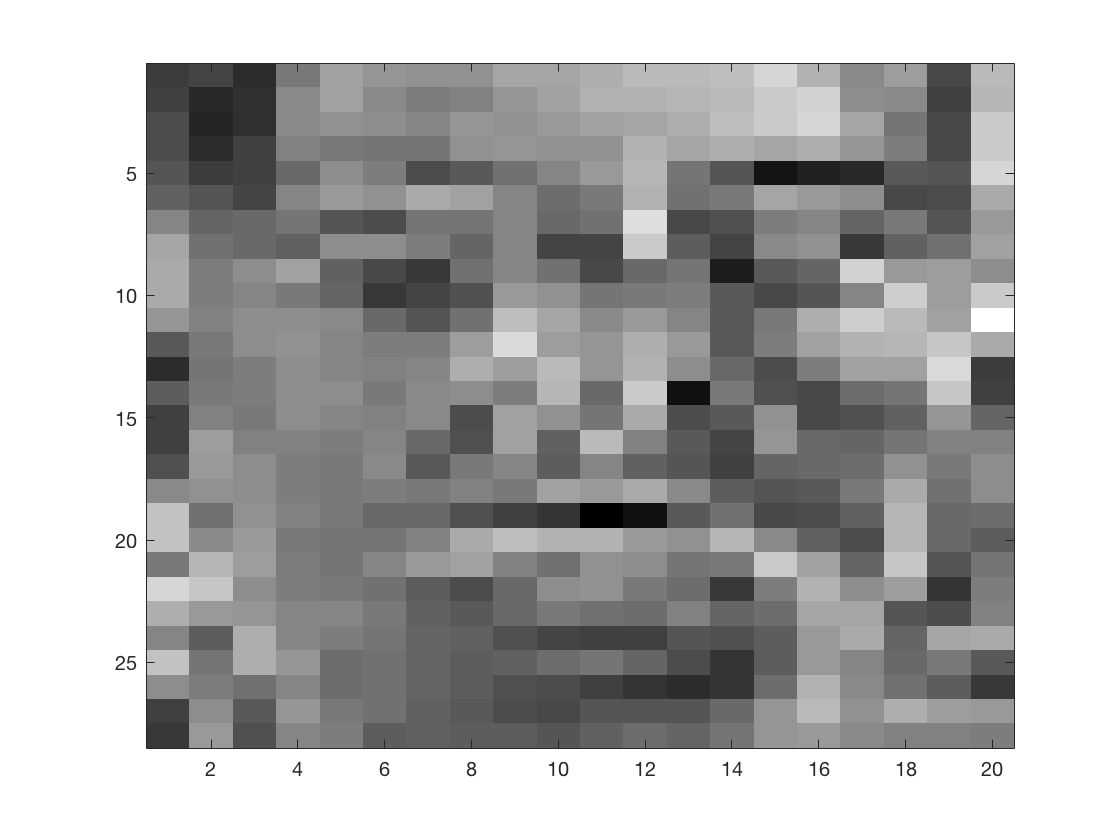
\includegraphics[scale=0.14]{4rand_re.png}
	}
	\caption{A Random Example}
	\label{fig-5}
\end{figure}

\subsubsection{Test with Noise}
Add extra noise to the informative example in \hyperref[sec-1.1.4]{Section~1.1.4}. See \hyperref[fig-6]{Figure~6}, and we will observe the effect of denoising by PCA.

\begin{figure}
	\centering
	\subfloat[Original]{
		\centering
		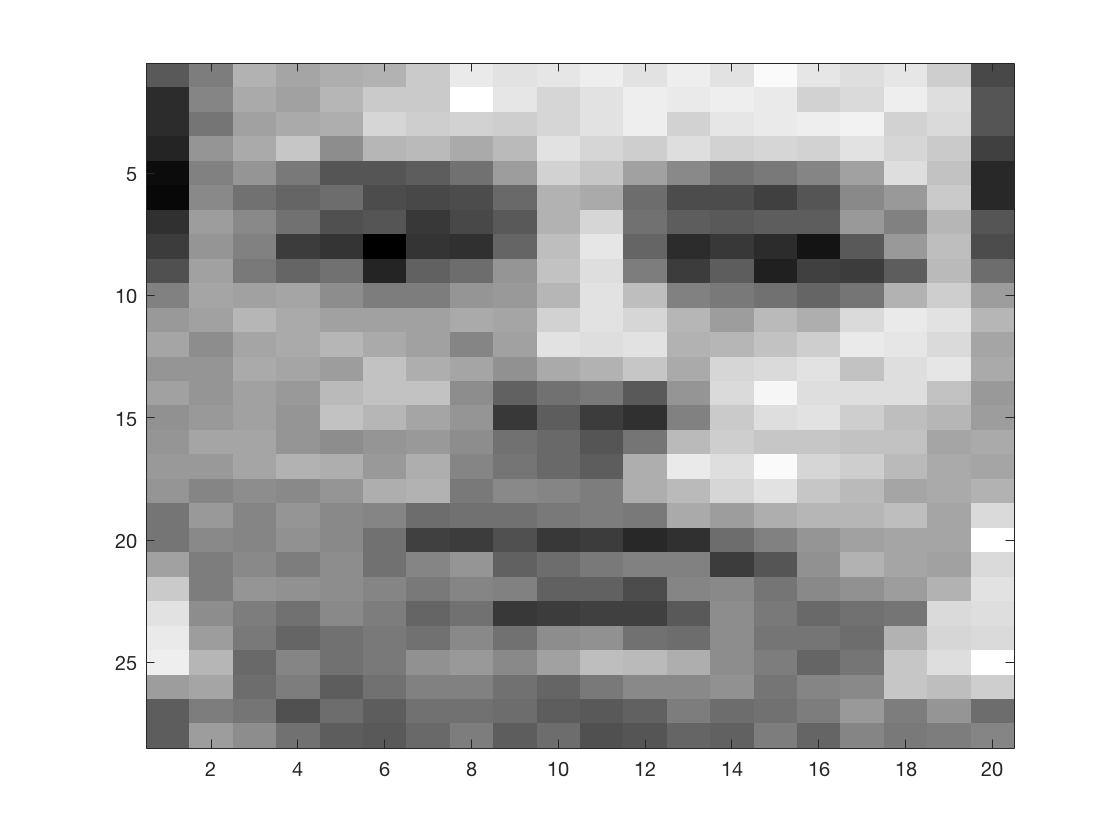
\includegraphics[scale=0.14]{4noise.png}
	}
	\quad
	\subfloat[Reconstructed]{
		\centering
		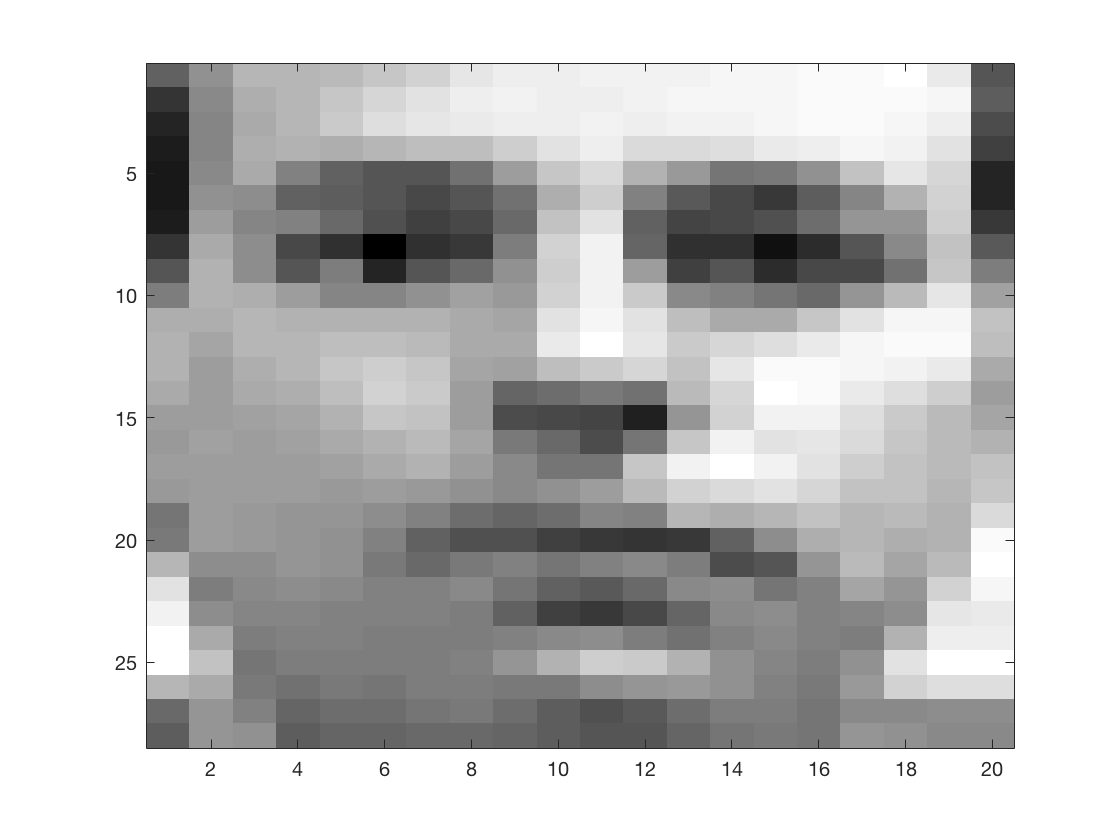
\includegraphics[scale=0.14]{4noise_re.png}
	}
	\caption{An Informative Example with Noise}
	\label{fig-6}
\end{figure}


\subsection{Isomap on Swiss Roll}
The code $swissroll.m$ provided by Roweis and Saul generates ``swiss roll'' data and runs LLE (Locally Linear Embedding) algorithm. I extract the data generation part of it and runs the isomap algorithm on the same data set. My script is called $swissroll\_isomap.m$. And the results are in \hyperref[fig-7]{Figure~7}.

\begin{figure}
	\centering
	\subfloat[]{
		\centering
		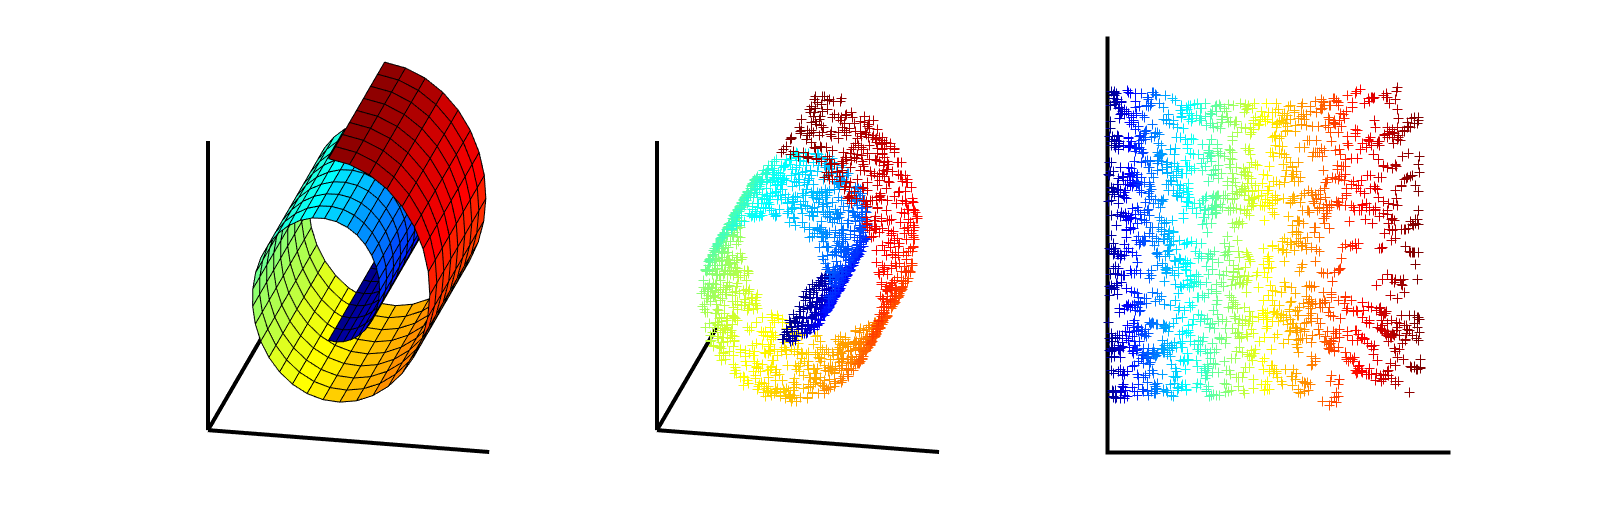
\includegraphics[scale=0.2]{isomap1.png}
	}

	\subfloat[]{
		\centering
		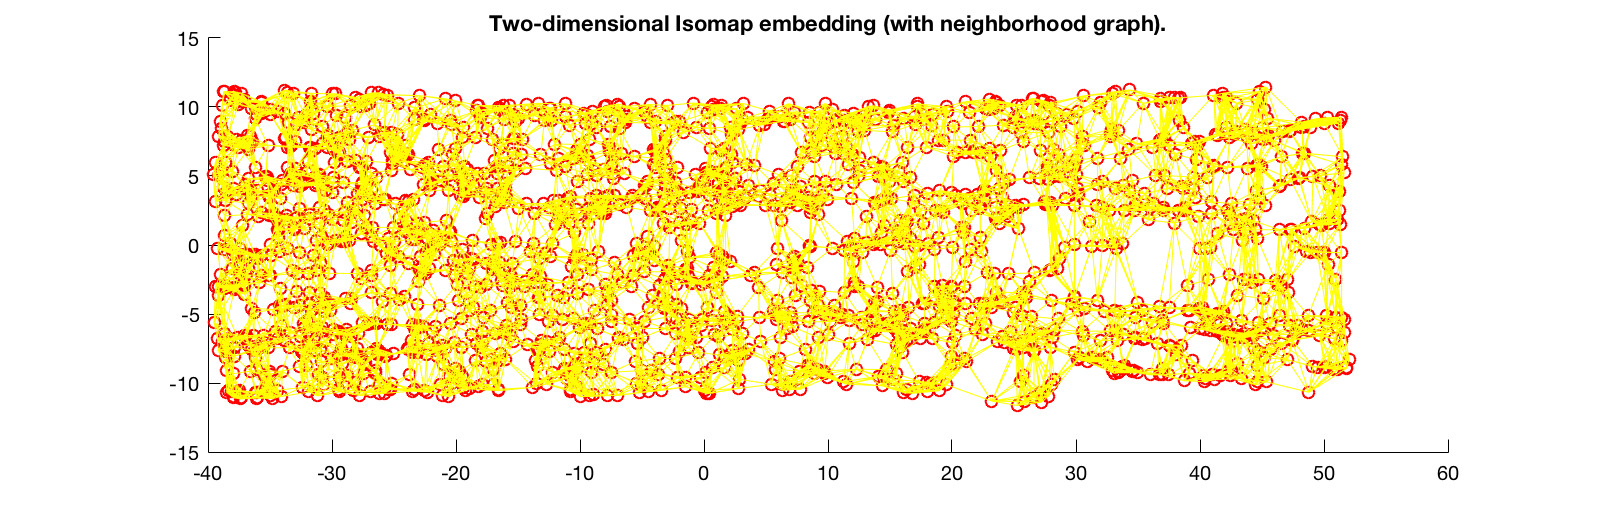
\includegraphics[scale=0.2]{isomap2.png}
	}
	\caption{Swiss Roll}
	\label{fig-7}
\end{figure}


\section{Gaussian Mixture Model}
\subsection{EM for Mixture of Gaussians}
When $\Sigma_k = \Sigma$ for all $k$, the expected complete-data log-likelihood function becomes
\[
\mathbb{E}_z[\ln p(x,z|\mu,\Sigma,\pi)] = \sum_{n=1}^N\sum_{k=1}^K\gamma(z_{nk})\{\ln \pi_k + \ln \mathcal{N}(x_k|\mu_k, \Sigma)\}
\]
where
\[
\gamma(z_{nk}) = \frac{\pi_k\mathcal{N}(x_n|\mu_k, \Sigma)}{\sum_{j=1}^K \pi_j\mathcal{N}(x_n|\mu_j,\Sigma)}
\]
Differentiating it w.r.t $\Sigma^{-1}$, we obtain
\[
\frac{N}{2} \Sigma - \frac{1}{2} \sum_{n=1}^N\sum_{k=1}^K\gamma(z_{nk})(x_n-\mu_k)(x_n-\mu_k)^T
\]
Note that we have used $\sum_{k=1}^K\gamma(z_{nk})=1$ for all $n$. Setting this to zero, we finally derive
\[
\Sigma = \frac{1}{N} \sum_{n=1}^N\sum_{k=1}^K\gamma(z_{nk})(x_n-\mu_k)(x_n-\mu_k)^T
\]
\subsection{Training}
We first experiment with $randConst$ in the function $mogEM$. I write script $setRandConst.m$ to plot $\log P(TrainingData)$ against $randConst$ (\hyperref[fig-8]{Figure~8}). As a result, $randConst = 1$ is a reasonable choice.

\begin{figure}
	\centering
	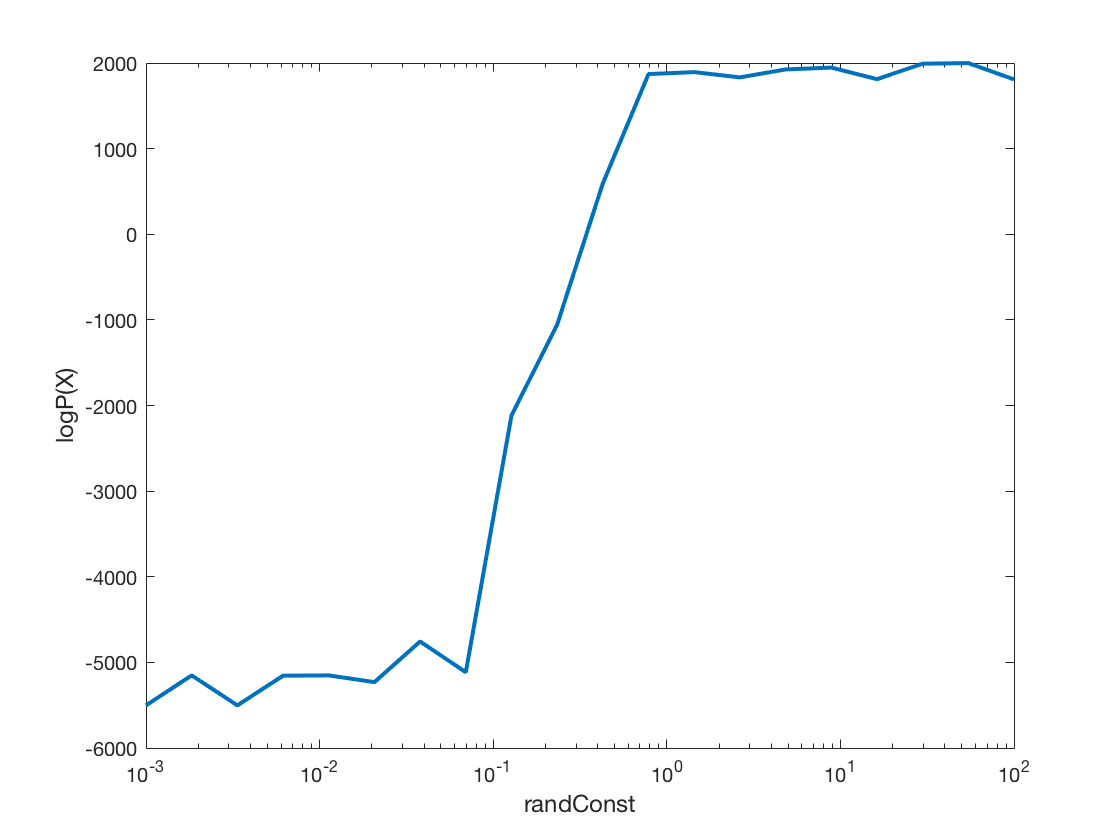
\includegraphics[scale=0.3]{randConst.png}
	\caption{$\log P(X)$ Against $randConst$}
	\label{fig-8}
\end{figure}

Run several times the below codes to train good models.
\begin{lstlisting}
[p2,mu2,vary2,logProbX3] = mogEM(train2,2,10,0.01,1);
[p3,mu3,vary3,logProbX3] = mogEM(train3,2,10,0.01,1);
\end{lstlisting}

The final model parameters are separately stored in $model2.mat$ and $model3.mat$.

Both the mean and variance vectors are shown as images in \hyperref[fig-9]{Figure~9} and \hyperref[fig-10]{Figure~10} using function $visualize\_digits$. The mixing proportions for the clusters within $model2$ are
\begin{verbatim}
p =

    0.4900
    0.5100
\end{verbatim}
The mixing proportions for the clusters within $model3$ are
\begin{verbatim}
p =

    0.4769
    0.5231
\end{verbatim}
Finally, $\log P(Training Data)$ is computed by
\begin{lstlisting}
sum(mogLogProb(p,mu,vary,x));
\end{lstlisting}
The results of two models are respectively
\begin{verbatim}
  -3.8202e+03
\end{verbatim}
and
\begin{verbatim}
   2.2582e+03
\end{verbatim}

\begin{figure}
	\centering
	\subfloat[Mean]{
		\centering
		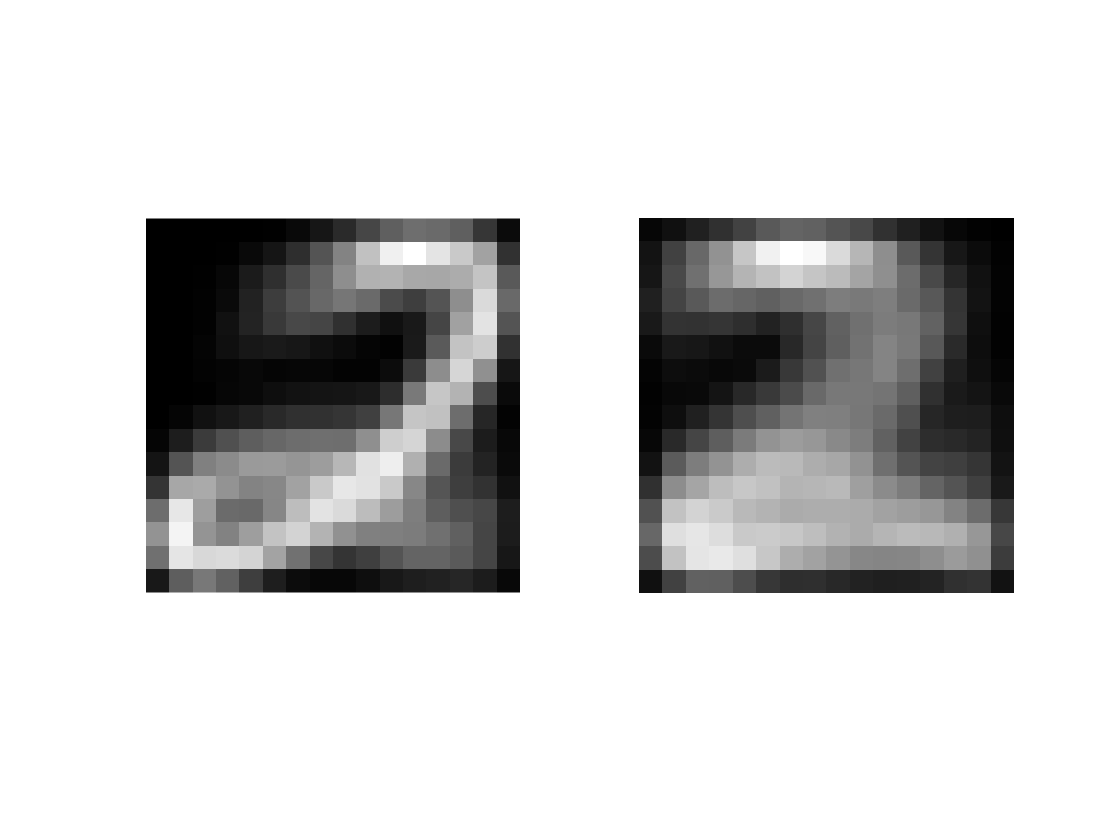
\includegraphics[scale=0.14]{model2_mu.png}
	}
	\quad
	\subfloat[Variance]{
		\centering
		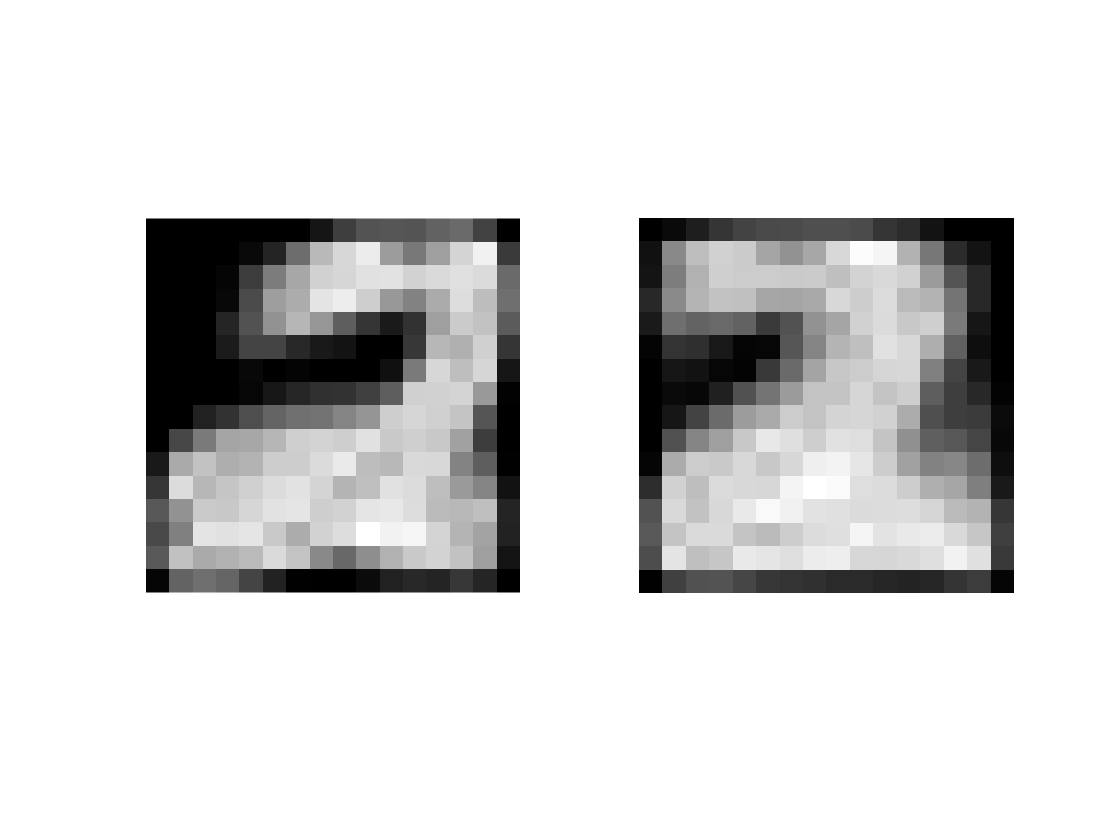
\includegraphics[scale=0.14]{model2_vary.png}
	}
	\caption{Mean and Variance of Model 2}
	\label{fig-9}
\end{figure}

\begin{figure}
	\centering
	\subfloat[Mean]{
		\centering
		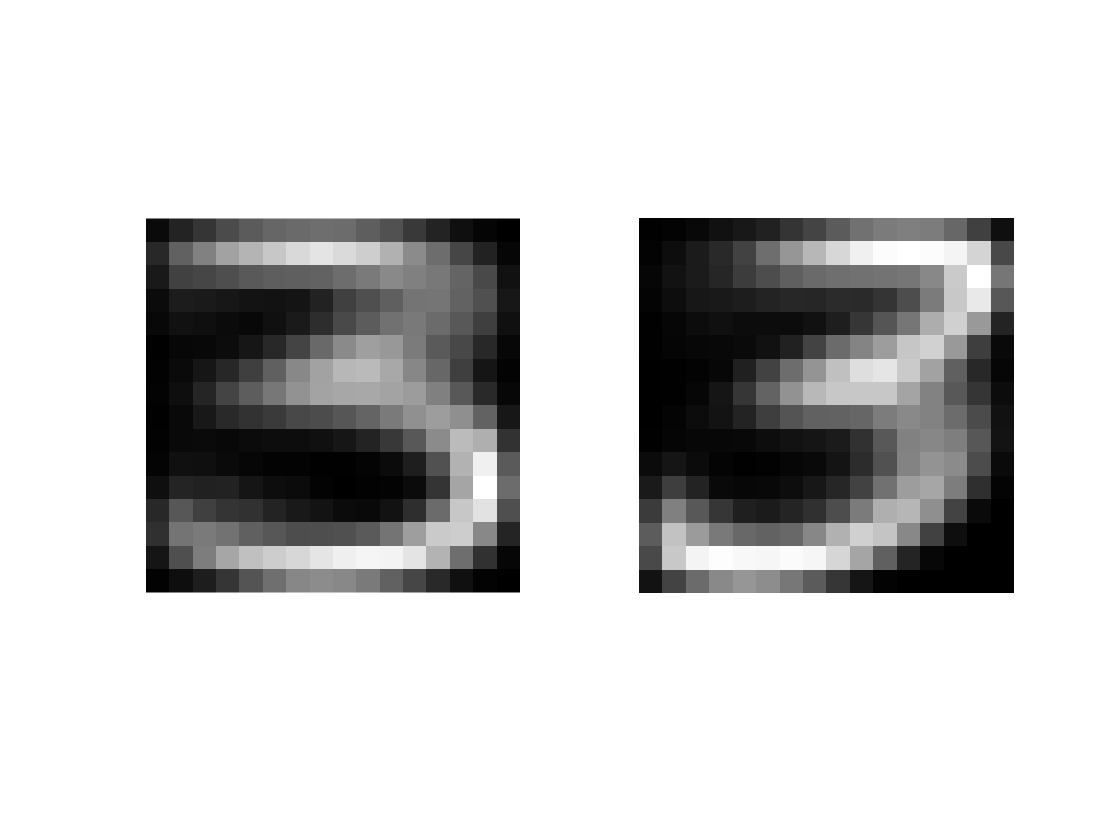
\includegraphics[scale=0.14]{model3_mu.png}
	}
	\quad
	\subfloat[Variance]{
		\centering
		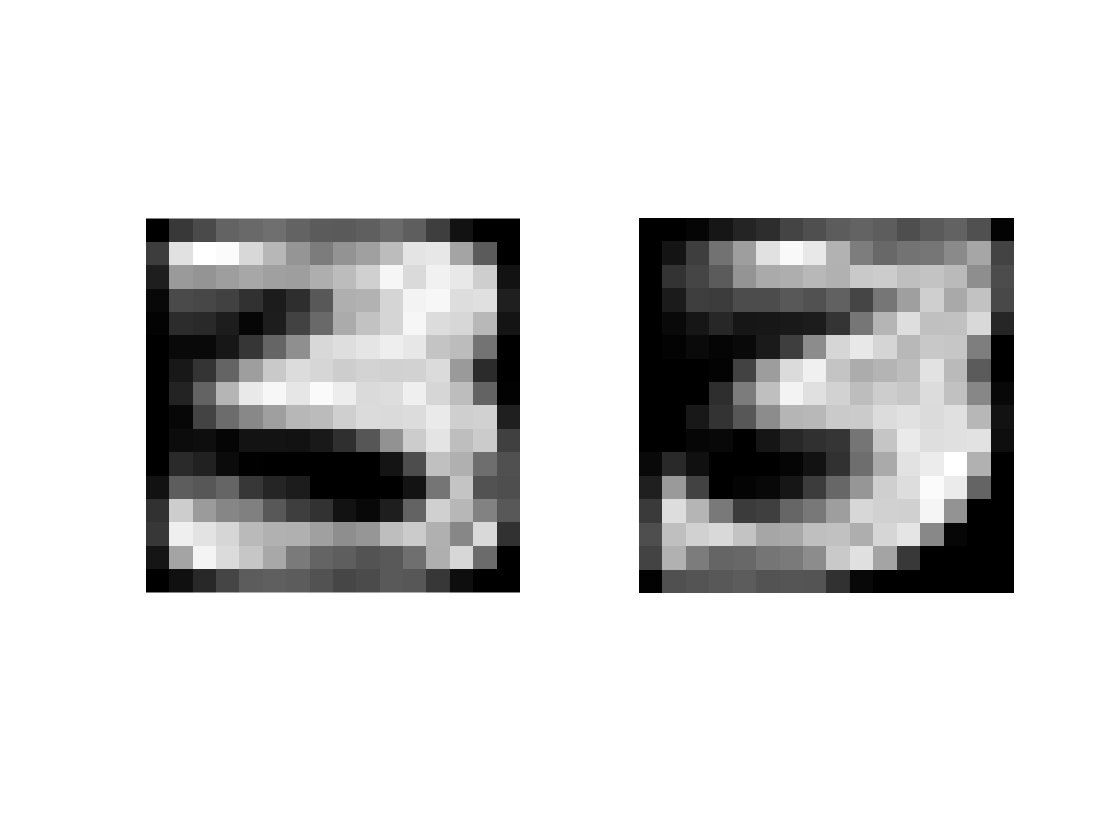
\includegraphics[scale=0.14]{model3_vary.png}
	}
	\caption{Mean and Variance of Model 3}
	\label{fig-10}
\end{figure}

\subsection{Initialize with K-Means}
Function $mogEM\_kmeans$ modified by me does the same thing as $mogEM$ does, except that $mu$ is initialized with k-means algorithm instead of in random.

Run $run\_q4.m$, and the results are stored in $q4.m$. The two converging processes with and without using k-means are shown in \hyperref[fig-11]{Figure~11}. Note that \hyperref[subfig-11(a)]{Figure~11(a)} converges at 5th iteration, whereas \hyperref[subfig-11(b)]{Figure~11(b)} only needs 2 iterations.

\begin{figure}
	\centering
	\subfloat[Original]{\label{subfig-11(a)}
		\centering
		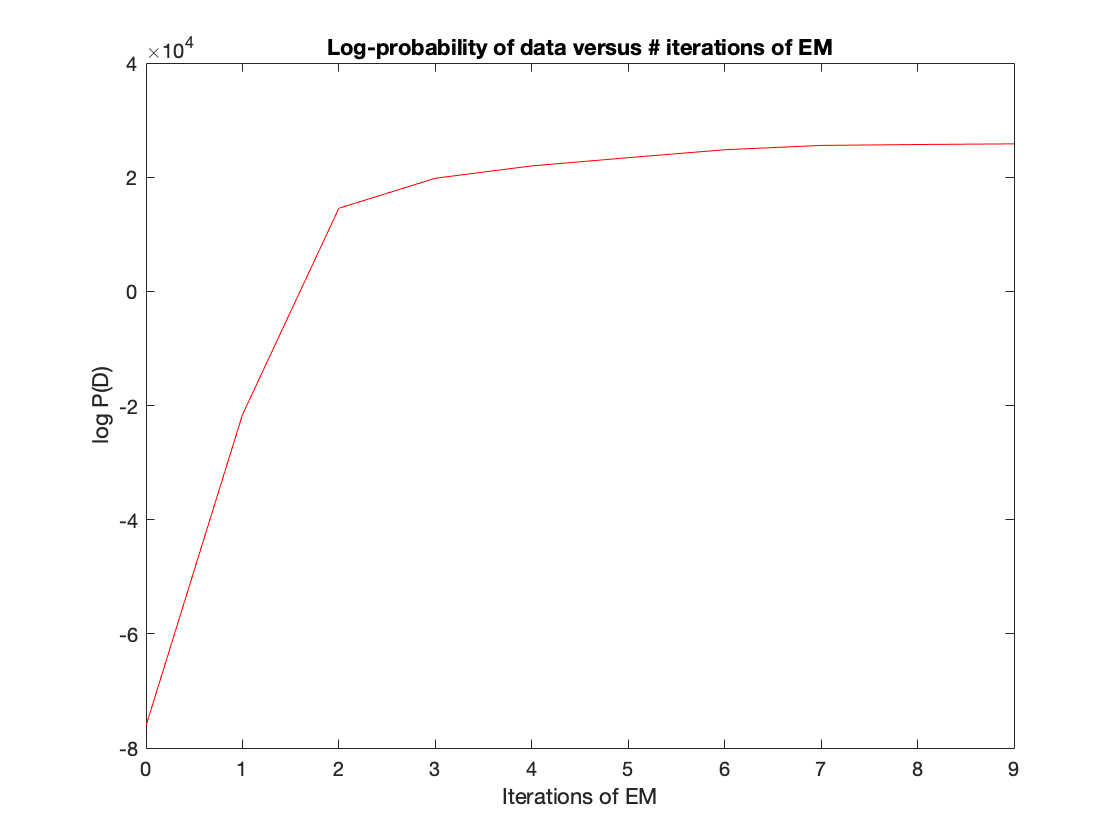
\includegraphics[scale=0.14]{q4_orig.png}
	}
	\quad
	\subfloat[K-Means]{\label{subfig-11(b)}
		\centering
		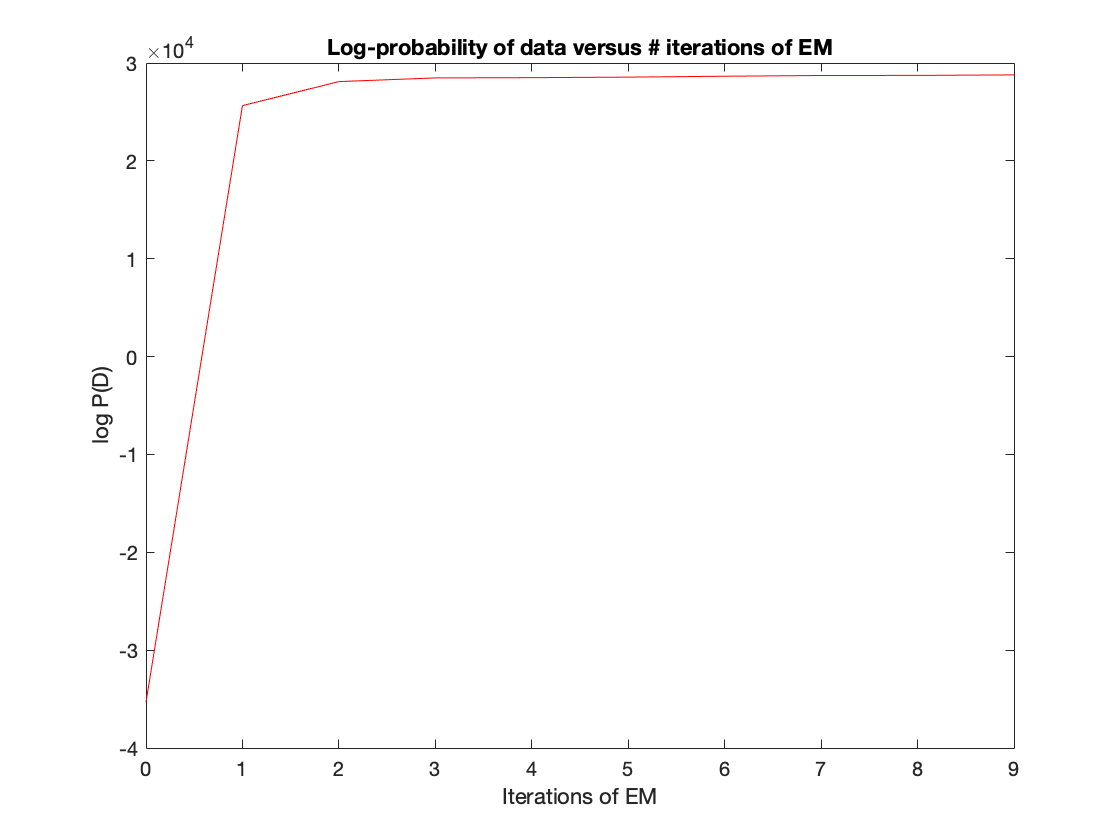
\includegraphics[scale=0.14]{q4_kmeans.png}
	}
	\caption{Converging Process}
	\label{fig-11}
\end{figure}

The final $log-prob$'s are separately
\begin{verbatim}
   2.4673e+04
\end{verbatim}
and
\begin{verbatim}
   2.7755e+04
\end{verbatim}

As a consequence, initializing with k-means algorithm provides much more efficiency, and is less likely to be trapped in local optimization.

\subsection{Classification Using MoGs}
$run\_q5.m$ plots the error rate against the number of clusters (\hyperref[fig-12]{Figure~12}). The model with each number of clusters has been trained for 20 times, and the error rate is computed averagely.

\begin{figure}
	\centering
	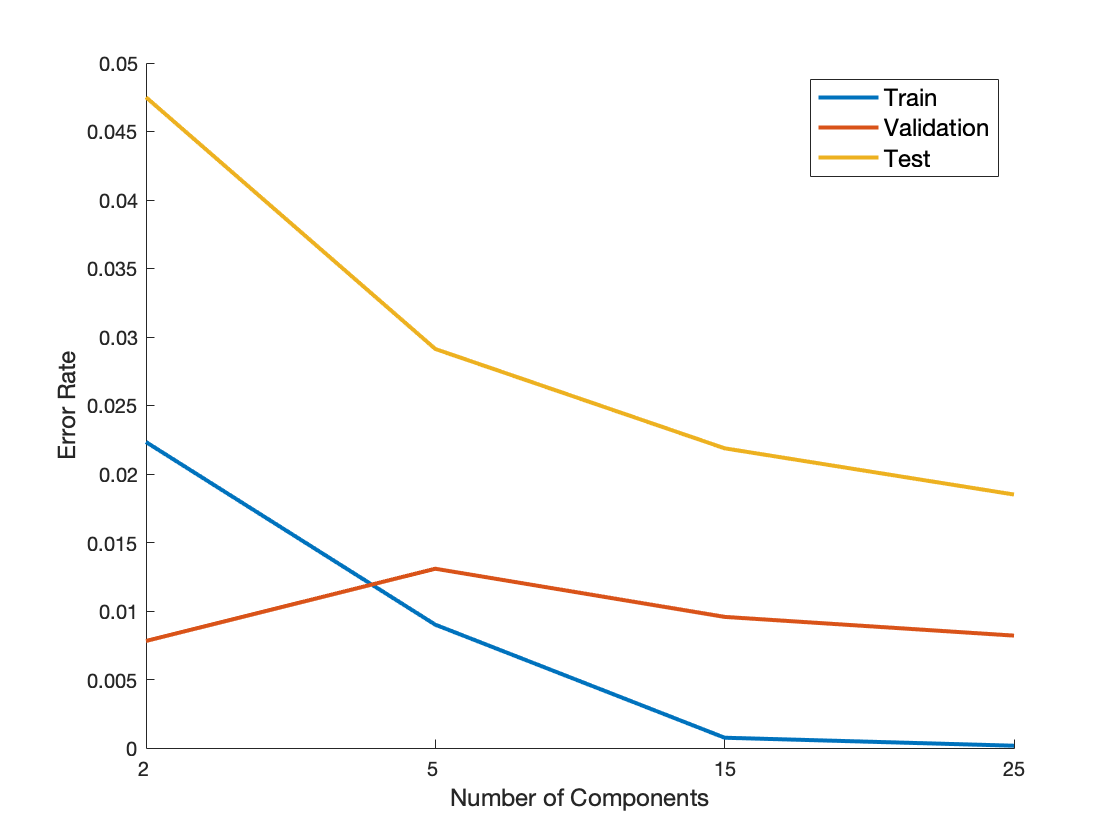
\includegraphics[scale=0.3]{q5.png}
	\caption{Error Rate}
	\label{fig-12}
\end{figure}

Answers:
\begin{enumerate}
	\item
	The error rates on the training sets generally decrease as the number of clusters increases, because more patterns are recognized. The more clusters, the more fitting for training data.
	\item
	The error rate curve for the test set decreases rapidly at the beginning, but slowly when the number of clusters is big. These phenomena---fitting and overfitting appear just like in any other machine learning models. A small number of clusters may not include enough necessary patterns, whereas too many clusters causes overfitting.
	\item
	If I wanted to choose a particular model as the best, I would certainly choose the 25-cluster model according to my above experiments. But if my aim is to achieve the lowest error rate possible on the new images my system will receive, which is obviously more meaningful, I will select the 15-cluster model as my final model. Because as we see in \hyperref[fig-12]{Figure~12}, there is no much difference between 15 and 20 clusters. In this way, we shall use 15 in order to avoid overfitting.
\end{enumerate}


\appendix
\section{MATLAB Codes}
\subsection{Dimensionality Reduction}
\subsubsection{\emph{select\_k.m}}
\begin{lstlisting}
% Edited by Yuanbo Han, Dec. 22, 2017.

load freyface.mat
X = double(X);  % convert to double

% Compute like SVD
N = size(X, 2);
[Vun, Dun] = eig(X*X'/N);
[lambda_un, order] = sort(diag(Dun));
Vun = Vun(:, order);
Xctr = X - repmat(mean(X, 2), 1, N);
[Vctr, Dctr] = eig(Xctr*Xctr'/N);
[lambda_ctr, order] = sort(diag(Dctr));
Vctr = Vctr(:, order);

% Eigen spectra (plot lambda_ctr)
figure;
plot(lambda_ctr, 'LineWidth', 1.5);
ylabel('\lambda', 'FontSize', 12);
title('Eigen spectra', 'FontSize', 15);

% Select k based on retention rate
original = sum(lambda_ctr);
new = 0;
r = 0.95;  % retention rate
for k=1:560
    new = new + lambda_ctr(end-k+1);
    if new / original >= r
        break;
    end
end
fprintf('k = %d, at the retention rate of %.2f%%\n', k, r*100);

\end{lstlisting}

\subsubsection{\emph{showEigenvectors.m}}
\begin{lstlisting}
% Show the top 16 eigenvectors with and without first removing the mean.
figure;
showfreyface(Vun(:,end-15:end));
figure;
showfreyface(Vctr(:,end-15:end));

\end{lstlisting}

\subsubsection{\emph{projectOnto2D.m}}
\begin{lstlisting}
% Project the data onto the top two eigenvectors,
% and plot the resulting 2D points.
Yctr = Vctr(:,end-1:end)' * X;
plot(Yctr(1,:), Yctr(2,:), '.');
explorefreymanifold(Yctr, X);

Yun = Vun(:,end-1:end)' * X;
plot(Yun(1,:), Yun(2,:), '.');
explorefreymanifold(Yun, X);

\end{lstlisting}

\subsubsection{\emph{PCAreconstruct.m}}
\begin{lstlisting}
function [X_re] = PCAreconstruct(Y,V)
% PCARECONSTRUCT(Y,V) compose the corresponding projected vector of Y,
% where V is the eigenvectors used in PCA.
%
% Edited by Yuanbo Han, Dec. 25, 2017.
X_re = V * Y;
end

\end{lstlisting}

\subsubsection{\emph{showReconstruct.m}}
\begin{lstlisting}
% Edited by Yuanbo Han, Dec. 25, 2017.

k = 80;
V = Vctr(:,end-k+1:end);

% Example for an original picture
figure;
showfreyface(X(:,50));  % the 50th sample in the data
figure;
showfreyface(PCAreconstruct(V'*(X(:,50)-mean(X,2)),V)+mean(X,2));

% Example for a random picture
R = randi([1,255], 560, 1);
figure;
showfreyface(R);
figure;
showfreyface(PCAreconstruct(V'*(R-mean(X,2)),V)+mean(X,2));

% Add noise for an original picture
X_noise = X(:,50) + 10*randn(560,1); % the 50th sample in the data
figure;
showfreyface(X_noise);
figure;
showfreyface(PCAreconstruct(V'*(X_noise-mean(X,2)),V)+mean(X,2));

\end{lstlisting}

\subsubsection{\emph{distmat.m}}
\begin{lstlisting}
function [dist] = distmat(p, q)
% function [dist] = distmat(v1, v2)
%
% Calculates pairwise distances between vectors. If v1 and v2 are both
% provided, a size(v1, 1) by size(v2, 1) matrix is returned, where the
% entry at (i,j) contains the Euclidean distance from v1(i,:) to v2(j,:).
% If only v1 is provided, squareform(pdist(v1)) is returned.

p = p';
if nargin == 1
    q = p;
else
    q = q';
end

[~, pn] = size(p);
[~, qn] = size(q);

pmag = sum(p .* p, 1);
qmag = sum(q .* q, 1);
dist = repmat(qmag, pn, 1) + repmat(pmag', 1, qn) - 2*p'*q;
dist = sqrt(dist);
end

\end{lstlisting}

\subsubsection{\emph{swissroll\_isomap.m}}
\begin{lstlisting}
% SWISS ROLL DATASET

N=2000;
K=12;
d=2;

clf; colordef none; colormap jet; set(gcf,'Position',[200,400,620,200]);

% PLOT TRUE MANIFOLD
tt0 = (3*pi/2)*(1+2*[0:0.02:1]); hh = [0:0.125:1]*30;
xx = (tt0.*cos(tt0))'*ones(size(hh));
yy = ones(size(tt0))'*hh;
zz = (tt0.*sin(tt0))'*ones(size(hh));
cc = tt0'*ones(size(hh));

subplot(1,3,1); cla;
surf(xx,yy,zz,cc);
view([12 20]); grid off; axis off; hold on;
lnx=-5*[3,3,3;3,-4,3]; lny=[0,0,0;32,0,0]; lnz=-5*[3,3,3;3,3,-3];
lnh=line(lnx,lny,lnz);
set(lnh,'Color',[1,1,1],'LineWidth',2,'LineStyle','-','Clipping','off');
axis([-15,20,0,32,-15,15]);

% GENERATE SAMPLED DATA
tt = (3*pi/2)*(1+2*rand(1,N));  height = 21*rand(1,N);
X = [tt.*cos(tt); height; tt.*sin(tt)];

% SCATTERPLOT OF SAMPLED DATA
subplot(1,3,2); cla;
scatter3(X(1,:),X(2,:),X(3,:),12,tt,'+');
view([12 20]); grid off; axis off; hold on;
lnh=line(lnx,lny,lnz);
set(lnh,'Color',[1,1,1],'LineWidth',2,'LineStyle','-','Clipping','off');
axis([-15,20,0,32,-15,15]); drawnow;

% RUN ISOMAP ALGORITHM
options.dims = 1:2;
Y = isomap(distmat(X'), 'k', K, options);

% SCATTERPLOT OF EMBEDDING
figure(1);
subplot(1,3,3); cla;
Y_2 = Y.coords{2};
scatter(Y_2(1,:),Y_2(2,:),12,tt,'+');
grid off;
set(gca,'XTick',[]); set(gca,'YTick',[]);

\end{lstlisting}

\subsection{Gaussian Mixture Model}
\subsubsection{\emph{mogEM\_test.m}}
\begin{lstlisting}
function [p,mu,vary,logProbX] = ...
    mogEM_test(x,K,iters,minVary,plotFlag,randConst)
% MOGEM_TEST does the same thing as MOGEM does, except that randConst can
% be initialized outside.
%
% Modifiedy by Yuanbo Han, Dec. 26, 2017.

if nargin==3 minVary = 0; plotFlag = 0; end
N = size(x,1); T = size(x,2);

plotString = cellstr(['bo'; 'gx'; 'r+'; 'c*'; 'ms'; 'yd'; 'kd']);
ellColor = ['b'; 'g'; 'r'; 'c'; 'm'; 'y'; 'k'];

% Initialize the parameters
%randConst = 1;
p = randConst+rand(K,1); p = p/sum(p);
mn = mean(x,2);
vr = std(x,[],2).^2;

%-------------------- Modify the code here ------------------------------
% Change the random initialization with k-means algorithm, use 5
% iterations.
mu = mn*ones(1,K)+randn(N,K).*(sqrt(vr)/randConst*ones(1,K));
%mu = kmeans(x,K,5);
%------------------------------------------------------------------------
vary = vr*ones(1,K)*2;
vary = (vary>=minVary).*vary + (vary<minVary)*minVary;

% Do iters iterations of EM
logProbX = zeros(iters,1);

for i=1:iters
    % Do the E step
    respTot = zeros(K,1); respX = zeros(N,K);
    respDist = zeros(N,K); logProb = zeros(1,T);
    ivary = 1./vary;
    logNorm = log(p)-0.5*N*log(2*pi)-0.5*sum(log(vary'),2);
    logPcAndx = zeros(K,T);
    for k=1:K
        logPcAndx(k,:) = logNorm(k) - 0.5*...
            sum((ivary(:,k)*ones(1,T)).*(x-mu(:,k)*ones(1,T)).^2,1);
    end
    [mx, mxi] = max(logPcAndx,[],1);
    PcAndx = exp(logPcAndx-ones(K,1)*mx); Px = sum(PcAndx,1);
    PcGivenx = PcAndx./(ones(K,1)*Px); logProb = log(Px) + mx;
    logProbX(i) = sum(logProb);
    
    % Plot log prob of data
    %{
  figure(1);
  set(gcf,'DoubleBuffer','on')
  clf;
  plot([0:i-1],logProbX(1:i),'r-');
  title('Log-probability of data versus # iterations of EM');
  xlabel('Iterations of EM');
  ylabel('log P(D)');
  drawnow;

  if plotFlag     % Plot the data and Gaussians
    figure(2);
    set(gcf,'DoubleBuffer','on')
    clf;
    hold on;
    for k=1:K
      plotEllipse(mu(1,k),mu(2,k),vary(1,k),vary(2,k),0,...
          ellColor(mod(k, length(ellColor))+1));
    end;
    for t=1:T  plot(x(1,t),x(2,t),...
            char(plotString(mod(mxi(t), length(plotString))+1))); end

    axis equal;
  end;
    %}
    
    respTot = mean(PcGivenx,2);
    respX = zeros(N,K); respDist = zeros(N,K);
    for k=1:K
        respX(:,k) = mean(x.*(ones(N,1)*PcGivenx(k,:)),2);
        respDist(:,k) = ...
            mean((x-mu(:,k)*ones(1,T)).^2.*(ones(N,1)*PcGivenx(k,:)),2);
    end
    
    % Do the M step
    p = respTot;
    mu = respX./(ones(N,1)*respTot'+eps);
    vary = respDist./(ones(N,1)*respTot'+eps);
    vary = (vary>=minVary).*vary + (vary<minVary)*minVary;
    
end
end

\end{lstlisting}

\subsubsection{\emph{setRandConst.m}}
\begin{lstlisting}
% Edited by Yuanbo Han, Dec. 26, 2017.
load digits.mat;

randConst = logspace(-3,2,20);
iters = 20;
repeat = 20;
logProbX_temp = zeros(iters,repeat);
logProbX = zeros(1,length(randConst));
for i = 1:length(randConst)
    fprintf('randConst = %f\n', randConst(i));
    for j = 1:repeat
        [~,~,~,logProbX_temp(:,j)] = ...
            mogEM_test(train3,2,iters,0.01,1,randConst(i));
        logProbX(i) = mean(logProbX_temp(end,:));
    end
    fprintf('logProbX = %f\n', logProbX(i));
end

figure;
semilogx(randConst, logProbX, 'LineWidth', 2);
xlabel('randConst', 'FontSize', 12);
ylabel('logP(X)', 'FontSize', 12);

\end{lstlisting}

\subsubsection{\emph{mogEM\_kmeans.m}}
\begin{lstlisting}
function [p,mu,vary,logProbX] = mogEM_kmeans(x,K,iters,minVary,plotFlag)
% MOGEM_KMEANS does the same thing as MOGEM does, except that mu is
% initialized with k-means algorithm instead of in random.
%
% Modifiedy by Yuanbo Han, Dec. 26, 2017.

if nargin==3
    minVary = 0;
    plotFlag = 0;
end

N = size(x,1); T = size(x,2);

plotString = cellstr(['bo'; 'gx'; 'r+'; 'c*'; 'ms'; 'yd'; 'kd']);
ellColor = ['b'; 'g'; 'r'; 'c'; 'm'; 'y'; 'k'];

% Initialize the parameters
randConst = 1;
p = randConst+rand(K,1); p = p/sum(p);
%mn = mean(x,2);
vr = std(x,[],2).^2;

%-------------------- Modify the code here ------------------------------
% Change the random initialization with k-means algorithm, use 5
% iterations.
%mu = mn*ones(1,K)+randn(N,K).*(sqrt(vr)/randConst*ones(1,K));
mu = kmeans(x,K,5);
%------------------------------------------------------------------------
vary = vr*ones(1,K)*2;
vary = (vary>=minVary).*vary + (vary<minVary)*minVary;

% Do iters iterations of EM
logProbX = zeros(iters,1);

for i=1:iters
    % Do the E step
    respTot = zeros(K,1); respX = zeros(N,K);
    respDist = zeros(N,K); logProb = zeros(1,T);
    ivary = 1./vary;
    logNorm = log(p)-0.5*N*log(2*pi)-0.5*sum(log(vary'),2);
    logPcAndx = zeros(K,T);
    for k=1:K
        logPcAndx(k,:) = logNorm(k)- 0.5*...
            sum((ivary(:,k)*ones(1,T)).*(x-mu(:,k)*ones(1,T)).^2,1);
    end
    [mx, mxi] = max(logPcAndx,[],1);
    PcAndx = exp(logPcAndx-ones(K,1)*mx); Px = sum(PcAndx,1);
    PcGivenx = PcAndx./(ones(K,1)*Px); logProb = log(Px) + mx;
    logProbX(i) = sum(logProb);
    
    % Plot log prob of data
    %{
  figure(1);
  set(gcf,'DoubleBuffer','on')
  clf;
  plot([0:i-1],logProbX(1:i),'r-');
  title('Log-probability of data versus # iterations of EM');
  xlabel('Iterations of EM');
  ylabel('log P(D)');
  drawnow;

  if plotFlag     % Plot the data and Gaussians
    figure(2);
    set(gcf,'DoubleBuffer','on')
    clf;
    hold on;
    for k=1:K
      plotEllipse(mu(1,k),mu(2,k),vary(1,k),vary(2,k),0,...
          ellColor(mod(k, length(ellColor))+1));
    end;
    for t=1:T  plot(x(1,t),x(2,t),...
            char(plotString(mod(mxi(t), length(plotString))+1))); end

    axis equal;
  end;
    %}
    
    respTot = mean(PcGivenx,2);
    respX = zeros(N,K); respDist = zeros(N,K);
    for k=1:K
        respX(:,k) = mean(x.*(ones(N,1)*PcGivenx(k,:)),2);
        respDist(:,k) = ...
            mean((x-mu(:,k)*ones(1,T)).^2.*(ones(N,1)*PcGivenx(k,:)),2);
    end
    
    % Do the M step
    p = respTot;
    mu = respX./(ones(N,1)*respTot'+eps);
    vary = respDist./(ones(N,1)*respTot'+eps);
    vary = (vary>=minVary).*vary + (vary<minVary)*minVary;
    
end
end

\end{lstlisting}

\subsubsection{\emph{run\_q4.m}}
\begin{lstlisting}
% Completed by Yuanbo Han, Dec. 26, 2017.
load digits;
x = [train2, train3];

% Train a MoG model with 20 components on all 600 training vectors
% with both original initialization and your kmeans initialization.

% Original initialization
[p1,mu1,vary1,logProbX1] = mogEM(x,20,10,0.01,0);
logProb1 = sum(mogLogProb(p1,mu1,vary1,x))

% K-means initialization
[p2,mu2,vary2,logProbX2] = mogEM_kmeans(x,20,10,0.01,0);
logProb2 = sum(mogLogProb(p2,mu2,vary2,x))

\end{lstlisting}

\subsubsection{\emph{run\_q5.m}}
\begin{lstlisting}
% Completed by Yuanbo Han, Dec. 26, 2017.
load digits;

errorTrain = zeros(1, 4);
errorValidation = zeros(1, 4);
errorTest = zeros(1, 4);
numComponent = [2, 5, 15, 25];
maxIter = 20; repeat = 20;

for i = 1 : 4
    K = numComponent(i);
    for r = 1:repeat
        % Train a MoG model with K components for digit 2
        [p2,mu2,vary2,~] = mogEM_kmeans(train2, K, maxIter, 0.01, 0);
        
        % Train a MoG model with K components for digit 3
        [p3,mu3,vary3,~] = mogEM_kmeans(train3, K, maxIter, 0.01, 0);
        
        % Caculate the probability P(d=1|x) and P(d=2|x),
        % classify examples, and compute the error rate
        % Hints: you may want to use mogLogProb function
        [inputs_train, inputs_valid, inputs_test, ...
            target_train, target_valid, target_test] = load_data();
        
        P2GivenTrain = mogLogProb(p2,mu2,vary2,inputs_train);
        P3GivenTrain = mogLogProb(p3,mu3,vary3,inputs_train);
        train_label = (P3GivenTrain > P2GivenTrain);
        errorTrain(i) = errorTrain(i) + 1/repeat * ...
            sum(train_label ~= target_train) / length(inputs_train);
        
        P2GivenValid = mogLogProb(p2,mu2,vary2,inputs_valid);
        P3GivenValid = mogLogProb(p3,mu3,vary3,inputs_valid);
        valid_label = (P3GivenValid > P2GivenValid);
        errorValidation(i) = errorValidation(i) + 1/repeat * ...
            sum(valid_label ~= target_valid) / length(inputs_valid);
        
        P2GivenTest = mogLogProb(p2,mu2,vary2,inputs_test);
        P3GivenTest = mogLogProb(p3,mu3,vary3,inputs_test);
        test_label = (P3GivenTest > P2GivenTest);
        errorTest(i) = errorTest(i) + 1/repeat * ...
            sum(test_label ~= target_test) / length(inputs_test);
    end
end

% Plot the error rate
figure;
hold on;
plot(1:4, errorTrain, 'LineWidth', 2);
plot(1:4, errorValidation, 'LineWidth', 2);
plot(1:4, errorTest, 'LineWidth', 2);
set(gca, 'XTick', 1:4);
set(gca, 'XTickLabel', numComponent);
lgd = legend({'Train','Validation','Test'}, 'Location', 'NorthEast');
set(lgd, 'FontSize', 12);
xlabel('Number of Components', 'FontSize', 12);
ylabel('Error Rate', 'FontSize', 12);

\end{lstlisting}

\end{document}